\documentclass{article}

\usepackage{amsmath}
\usepackage{amscd}
\usepackage[tableposition=top]{caption}
\usepackage{ifthen}
\usepackage[utf8]{inputenc}

\usepackage{Sweave}
\begin{document}

\title{Estimating HIV transmission rates with \texttt{rcolgem}}
\author{Erik M Volz}
\date{\today}
\maketitle

This vignette will demonstrate how to use structured coalescent models\cite{volz2012complex} to estimate epidemiological parameters given a pathogen genealogy and discrete-trait information about sampled individuals. 
We will focus on the problem of estimating HIV transmission rates by stage of infection and assuming we know the stage of infection when patients are sampled and virus is sequenced. 

We will fit a very simple model of an HIV epidemic using ordinary differential equations. 
In this model, the infectious period will be broken into three stages of different average duration and with different transmission rates. 
The first stage, \emph{early HIV infection} (EHI) is short (average duration $1/\gamma_0$=1 year), but has high transmission rate $\beta_0$. 
The second stage, \emph{chronic HIV infection}, is long (average duration $1/\gamma_1$=7 years), and has small transmission rate. 
The last stage, AIDS, lasts $1/\gamma_2=2$ years on average and has an intermediate transmission rate.
There are births into the susceptible state at rate $b N$ where $N=S + I_0 + I_1 + I_2$. 
And there is mortality due to natural causes from all states at rate $\mu$. 
The parameter values are listed in table~\ref{tab:parms}. 
The model equations are as follows: 
\begin{align}
	\dot{S} &= b N - \mu S - (\beta_0 I_0 + \beta_1 I_1 + \beta_2 I_2) S / N  \\
	\dot{I_0} &= (\beta_0 I_0 + \beta_1 I_1 + \beta_2 I_2) S / N - (\mu + \gamma_0) I_0  \\
	\dot{I_1} &= \gamma_0 I_0 - (\mu + \gamma_1) I_1  \\
	\dot{I_2} &= \gamma_1 I_1 - (\mu + \gamma_2) I_2 
\end{align}
The model is also illustrated in figure~\ref{fig:hivmodel}.

\begin{table}
\caption{ Parameter symbols and values. \label{tab:parms} }
\begin{center}
	\begin{tabular}{lll}
		\hline 
		Parameter & Symbol & Value \\
		\hline
		Duration EHI & $1/\gamma_0$ & 1 year \\
		Duration chronic & $1/\gamma_1$ & 7 years \\
		Duration AIDS & $1/\gamma_2$  & 2 years \\
		Birth rate & $b$ & 0.036 \\
		Natural death rate & $\mu$ &  1/30 \\
		EHI transmission rate & $\beta_0$ & 1.2 \\
		Chronic transmission rate & $\beta_1$ & 0.03 \\
		AIDS transmission rate  &  $\beta_2$ & 0.09 \\
		Initial no. susceptibles & $S(0)$ & 3000 \\
		\hline 
	\end{tabular}
\end{center}
\end{table}

The package is loaded by
\begin{Schunk}
\begin{Sinput}
> library(rcolgem)
\end{Sinput}
\end{Schunk}

Create a list of the true parameter values: 
\begin{Schunk}
\begin{Sinput}
> parms_truth <- list(gamma0 = 1
+  , gamma1 = 1/7
+  , gamma2 = 1/2
+  , mu = 1/30
+  , b=.036
+  , beta0 = 12./10
+  , beta1=3./100
+  , beta2=9./100
+  , S_0=3000
+  , I0_0=1, I1_0=0.01, I2_0=0.01
+  , m=3, mm=1) 
\end{Sinput}
\end{Schunk}

\begin{figure}
\begin{center}
	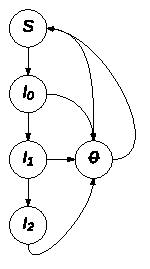
\includegraphics[width=.4\textwidth]{figure/siiirs.pdf}
\end{center}
	\caption{ An illustration of the HIV compartmental model. \label{fig:hivmodel}}
\end{figure}


In order to fit this model, we need to express the equations in a canonical format. 
According to this format, we will tally birth and migration events between demes. 
In our example, the deme corresponds to the stage of infection that an infected host can be in, so we will refer the demes with the following names:
\begin{Schunk}
\begin{Sinput}
> INFECTEDNAMES <- c('I0', 'I1', 'I2')
\end{Sinput}
\end{Schunk}

There are $m=3$ demes in this model, so the birth events between demes needs to be expressed with a $3\times 3$ matrix $F$. 
The element $F_{kl}$ represents the rate of transmissions by a host in deme $k$ to a host in deme $l$. 
In our example, this is the following:
\begin{Schunk}
\begin{Sinput}
> births <- rbind( 
+   c('parms$beta0 * S * I0 / (S + I0 + I1 + I2)', '0', '0'), 
+   c('parms$beta1 * S * I1 / (S + I0 + I1 + I2)', '0', '0'), 
+   c('parms$beta2 * S * I2 / (S + I0 + I1 + I2)', '0', '0')
+ )
> rownames(births)=colnames(births)<- INFECTEDNAMES
\end{Sinput}
\end{Schunk}
Each element of the matrix is a string that will be parsed as R code and evaluated, so it is important to write it exactly as you would if you were solving the equations outside of colgem.
Also note that the object \texttt{parms} is accessible to these equations, which is a list of parameters- this may include parameters to be estimated.
Note that there are zero rates in the 2nd and third columns, since all new infected hosts start out in the first stage of infection (EHI). 
Also note that we \emph{must} give row and column names to the matrix, and these names must correspond to the names of the demes. 

Similarly, we must create a matrix of migrations:
\begin{Schunk}
\begin{Sinput}
> migrations <- rbind(
+   c('0', 'parms$gamma0 * I0', '0'),
+   c('0', '0', 'parms$gamma1 * I1'),
+   c('0', '0', '0')
+ )
> rownames(migrations)=colnames(migrations) <- INFECTEDNAMES
\end{Sinput}
\end{Schunk}
Note that this matrix tallys the stage progression from EHI to chronic and from chronic to AIDS. 

We must also write a vector of expressions for events that terminate a lineage-- In this model, this occurs due to natural or AIDS related mortality: 
\begin{Schunk}
\begin{Sinput}
> deaths <- c(
+  'parms$mu*I0'
+  , 'parms$mu*I1'
+  , 'parms$mu*I2 + parms$gamma2 * I2'
+ )
> names(deaths) <- INFECTEDNAMES
\end{Sinput}
\end{Schunk}

Finally, we must write a vector of ODEs for state variables that do not correspond to demes in the coalescent model. 
In our example, there is only one such variable- the number of susceptibles: 
\begin{Schunk}
\begin{Sinput}
> nonDemeDynamics <- paste(sep='',
+ '-parms$mu*S + parms$mu*(S + I0 + I1 + I2)'
+  ,'- S * (parms$beta0*I0+parms$beta1*I1+parms$beta2*I2) / (S + I0 + I1 + I2)'
+ )
> names(nonDemeDynamics) <- 'S'
\end{Sinput}
\end{Schunk}
Note well that in all cases, the expression or equation must have the corresponding name of the state variable. 

The model can be fitted to a binary tree with dated tips. 
We will use a simulated tree such that we know the true parameter values and population size through time. 
We load this by: 
\begin{Schunk}
\begin{Sinput}
> # read the tree
> tree <- read.tree(
+    system.file('extdata/hivSimulation.nwk', package='rcolgem'))
> #~ the sample times are the same, because it is a homochronous sample at 50 years
> sampleTimes <- rep(50, length(tree$tip.label))
> names(sampleTimes) <- tree$tip.label
> # create a tree with dated tips and internal nodes, 
> # will infer the sample states from tip labels
> bdt <- binaryDatedTree(tree
+   , sampleTimes
+   , sampleStatesAnnotations=INFECTEDNAMES)
> bdt
\end{Sinput}
\begin{Soutput}
Phylogenetic tree with 318 tips and 317 internal nodes.

Tip labels:
	89_I1, 349_I2, 339_I1, 64_I1, 203_I1, 30_I0, ...

Rooted; includes branch lengths.
\end{Soutput}
\end{Schunk}
Note well that the vector of sample times must have the names of each taxon. 
If the state of each taxon (the stage of infection of each sample unit) is encoded at the end of taxon name, it can be loaded automatically by passing the argument \texttt{sampleStatesAnnotations}.  
Alternatively, that information can be passed as a matrix with row names corresponding to the tip labels of the tree. 

Now we can calculate the likelihood of the tree and see how long it takes:
\begin{Schunk}
\begin{Sinput}
> print(system.time( print(
+ 	coalescent.log.likelihood( bdt
+ 	 , births,  deaths, nonDemeDynamics
+ 	 , t0 = 0
+ 	 , x0=c(I0=1, I1=.01, I2=.01, S = parms_truth$S_0)
+ 	 , migrations = migrations
+ 	 , parms=parms_truth
+ 	 , fgyResolution=1000
+ 	 , integrationMethod='euler'
+ 	)
+ )))
\end{Sinput}
\begin{Soutput}
[1] -2214.567
   user  system elapsed 
  1.580   0.004   1.590 
\end{Soutput}
\end{Schunk}
It's a bit slow, so note that there is an alternative low-level interface that can be a bit faster (\texttt{coalescent.log.likelihood.fgy}). Also note that changing the \texttt{integrationMethod} (choose `euler'), \texttt{censorAtHeight} (only fit to part of the tree) and \texttt{fgyResolution} (set to a smaller value) options can dramatically speed up the calculation at the cost of some accuracy. 

We can fit the model by using the \texttt{bbmle} or \texttt{stats4} package. 
\begin{Schunk}
\begin{Sinput}
> library(bbmle)
\end{Sinput}
\end{Schunk}
We will focus on estimating the three transmission rates of the system along with a nuisance parameter that controls initial conditions, $t_0$, which is the time of origin of the epidemic. We will assume prior knowledge of the stage progression rates $\gamma_i$ mortality rates $\mu$, and susceptible population size $S(0)$.


First, create the objective function to be minimized:
\begin{Schunk}
\begin{Sinput}
> obj_fun <- function(lnbeta0, lnbeta1, lnbeta2, t0)
+ {
+ 	parms <- parms_truth
+ 	parms$beta0 <- exp(lnbeta0)
+ 	parms$beta1 <- exp(lnbeta1)
+ 	parms$beta2 <- exp(lnbeta2)
+ 	mll <- -coalescent.log.likelihood( bdt
+ 		 , births, deaths, nonDemeDynamics
+ 		 , t0 = t0
+ 		 , x0=c(I0=1, I1=.01, I2=.01, S = parms$S_0)
+ 		 , migrations = migrations
+ 		 , parms=parms
+ 		 , fgyResolution = 1000
+ 		 , integrationMethod = 'rk4'
+ 	)
+ 	# track progress: 
+ 	print(c(mll, exp(c(lnbeta0, lnbeta1, lnbeta2) ), t0) )
+ 	mll
+ }
\end{Sinput}
\end{Schunk}
Note that this uses log-transformation for variables that must be positive (like rates).

We can then fit the model by running
\begin{Schunk}
\begin{Sinput}
> fit <- mle2(obj_fun
+   , start=list(lnbeta0=log(.6), lnbeta1=log(.2), lnbeta2=log(.05), t0=0)
+   , method='Nelder-Mead', optimizer='optim' 
+   ,  control=list(trace=6, reltol=1e-8))
\end{Sinput}
\end{Schunk}
Note that we are starting the optimizer far from the true parameter values.
If fitting a model to real data, it is recommended to try many different starting conditions over a large range of values.  
The optimizer would take about 10 minutes to run, so instead we will load the results:
\begin{Schunk}
\begin{Sinput}
> load( system.file('extdata/hivModel0-fit.RData', package='rcolgem') )
> AIC(fit)
\end{Sinput}
\begin{Soutput}
[1] 4447.468
\end{Soutput}
\begin{Sinput}
> logLik(fit)
\end{Sinput}
\begin{Soutput}
'log Lik.' -2219.734 (df=4)
\end{Soutput}
\begin{Sinput}
> coef(fit)
\end{Sinput}
\begin{Soutput}
   lnbeta0    lnbeta1    lnbeta2         t0 
 0.1772788 -3.3862403 -2.9639203 -1.8339507 
\end{Soutput}
\begin{Sinput}
> exp(coef(fit))
\end{Sinput}
\begin{Soutput}
   lnbeta0    lnbeta1    lnbeta2         t0 
1.19396395 0.03383565 0.05161617 0.15978107 
\end{Soutput}
\end{Schunk}


We can compare the fitted model to the true number of infected through time, which is shown in figure~\ref{fig:results0}
\begin{figure}
	\begin{center}
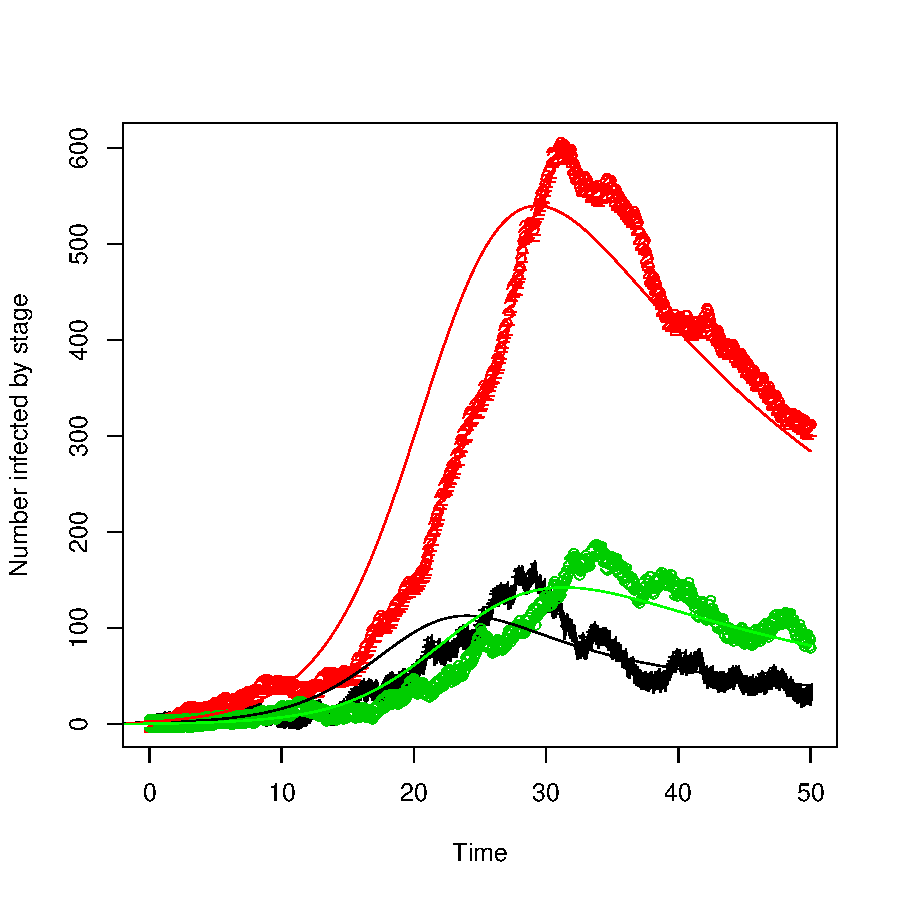
\includegraphics{hiv_vignette-results0}
	\end{center}
	\caption{The actual (points) and estimated (lines) number of infections through time. Black: EHI, Red:chronic, Green:AIDS. 
		\label{fig:results0}}
\end{figure}



We can calculate a confidence interval for the transmission rates using likelihood profiles:
\begin{Schunk}
\begin{Sinput}
> profbeta <- profile(fit, which=1, alpha=.05
+ 	, std.err=.5, trace=TRUE, tol.newmin=1 )
\end{Sinput}
\end{Schunk}
This takes a long time, so we will load the results:
\begin{Schunk}
\begin{Sinput}
> load( system.file('extdata/hivModel0-profbeta.RData',  package='rcolgem') )
\end{Sinput}
\end{Schunk}
We see that the confidence interval covers the true value:
\begin{Schunk}
\begin{Sinput}
> c( exp( confint( profbeta ) ), TrueVal=parms_truth$beta0 )
\end{Sinput}
\begin{Soutput}
   2.5 %   97.5 %  TrueVal 
1.093873 1.243095 1.200000 
\end{Soutput}
\end{Schunk}
And, we can visualize the profile (Figure~\ref{fig:profile}). 
\begin{Schunk}
\begin{Sinput}
> plot(profbeta)
> abline( v = log( parms_truth$beta0) , col='red')
\end{Sinput}
\end{Schunk}
\begin{figure}
\begin{center}
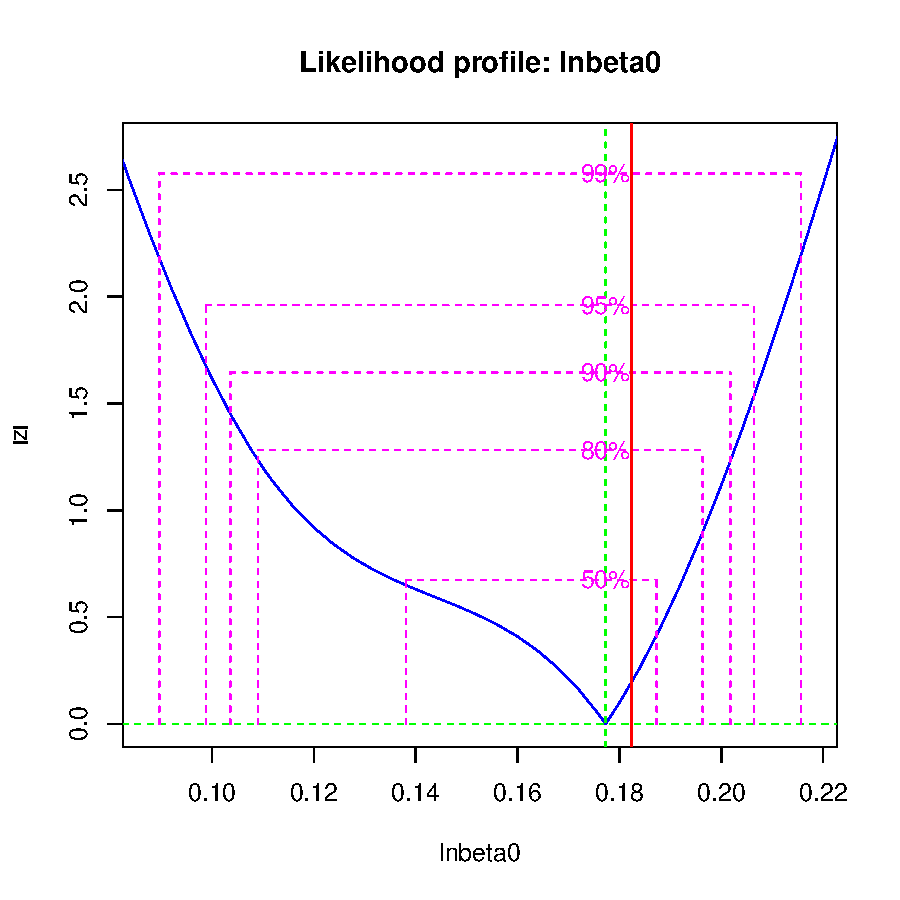
\includegraphics{hiv_vignette-proffigure}
\end{center}
\caption{Likelihood profile for the transmission rate $\beta_0$ with confidence levels. The true parameter value is indicated by the vertical red line.\label{fig:profile}}
\end{figure}



\bibliographystyle{plain}
\bibliography{hiv_vignette}
\end{document}
